\documentclass[11pt,border=5pt]{standalone}
\usepackage{fontspec}
\setmainfont{cmunrm.otf}[BoldFont=cmunbx.otf,ItalicFont=cmunti.otf,BoldItalicFont=cmunbi.otf]
\usepackage{amsmath}
\usepackage{unicode-math}
\setmathfont{NewCMMath-Regular.otf}
\usepackage{tikz}
\usetikzlibrary{arrows.meta,patterns,angles,quotes}
\begin{document}
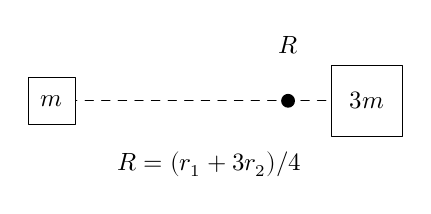
\begin{tikzpicture}[>=Stealth,font=\small,line cap=round,line join=round]
\draw[dashed] (-2,0) -- (2,0);
\draw[fill=white] (-2.3,-0.3) rectangle (-1.7,0.3);
\node at (-2,0) {$m$};
\draw[fill=white] (1.55,-0.45) rectangle (2.45,0.45);
\node at (2,0) {$3m$};
\fill (1,0) circle (2.5pt);
\node at (1,0.7) {$R$};
\node at (0,-0.8) {$R=(r_1+3r_2)/4$};

\end{tikzpicture}
\end{document}
